\documentclass[aspectratio=169]{beamer}

% ---------- Theme & Colors ----------
\usetheme{Madrid}
\usecolortheme{seahorse}
\definecolor{deepblue}{RGB}{13,71,161}
\definecolor{softgreen}{RGB}{46,125,50}
\setbeamercolor{title}{fg=white,bg=deepblue}
\setbeamercolor{frametitle}{fg=white,bg=deepblue}
\setbeamercolor{block title}{bg=softgreen,fg=white}
\setbeamercolor{block body}{bg=softgreen!10}
\setbeamercolor{item}{fg=deepblue}
\setbeamertemplate{navigation symbols}{}
\setbeamertemplate{footline}{
  \leavevmode\hbox{%
    \begin{beamercolorbox}[wd=.33\paperwidth,ht=2.5ex,dp=1ex,center]{author in head/foot}%
      \usebeamerfont{author in head/foot}\insertshortauthor
    \end{beamercolorbox}%
    \begin{beamercolorbox}[wd=.34\paperwidth,ht=2.5ex,dp=1ex,center]{title in head/foot}%
      \usebeamerfont{title in head/foot}\insertshorttitle
    \end{beamercolorbox}%
    \begin{beamercolorbox}[wd=.33\paperwidth,ht=2.5ex,dp=1ex,right]{date in head/foot}%
      \insertframenumber{} / \inserttotalframenumber\hspace*{2ex}
    \end{beamercolorbox}}%
}

% ---------- Packages ----------
\usepackage{graphicx}
\usepackage{booktabs}
\usepackage{hyperref}
\usepackage{tikz}
\usetikzlibrary{shapes.geometric, arrows.meta, positioning}

% ---------- Title Info ----------
\title[Rainfall Prediction]{Rainfall Prediction System Using Machine Learning}
\subtitle{Next-Day Rain Prediction for Australian Weather Stations}
\author[Yati Singh]{Yati Singh\texorpdfstring{\\}{ -- }\small Roll No.: E23CSEU1058}
\institute[Bennett University]{Bennett University, Noida\texorpdfstring{\\[0.3em]}{ -- }CSET 431: Special Topics in Computer Science}
\titlegraphic{
\includegraphics[height=1.8cm]{images/bu_logo.png}}
\date{}

% ========================================================
\begin{document}

% -------------------- Slide 1: Title --------------------
{
\setbeamertemplate{footline}{}
\begin{frame}[noframenumbering]
  \vfill
  \centering
  \begin{beamercolorbox}[sep=8pt,center,rounded=true]{title}
    {\Large\bfseries Rainfall Prediction System Using Machine Learning}\\[0.3em]
    {\normalsize Next-Day Rain Prediction for Australian Weather Stations}
  \end{beamercolorbox}
  \vspace{1em}
  
\includegraphics[height=2.0cm]{images/bu_logo.png}\\[0.6em]
  {\large\textbf{Bennett University, Noida}}\\[0.2em]
  {\normalsize CSET 431: Special Topics in Computer Science}\\[1em]
  {\normalsize Yati Singh}\\[0.2em]
  {\small Roll No.: E23CSEU1058}
  \vfill
\end{frame}
}

% -------------------- Slide 2: Introduction & Motivation --------------------
\begin{frame}{Introduction \& Motivation}
  \begin{columns}[T]
    \begin{column}{0.55\textwidth}
      \begin{itemize}
        \item Over 80\% of Australia receives $<$600\,mm annual rainfall --- accurate forecasting is critical.
        \item \textbf{Objective:} Predict whether it will \textbf{rain tomorrow} at a given Australian location using current-day weather observations.
        \item \textbf{Dataset:} \emph{Rain in Australia} (Kaggle) --- $\sim$145\,k observations across \textbf{49 stations} (2007--2017).
        \item \textbf{Target:} \texttt{RainTomorrow} (Yes / No).
      \end{itemize}
    \end{column}
    \begin{column}{0.42\textwidth}
      \begin{block}{Key Challenge}
        Dataset is \textbf{highly imbalanced}: only $\sim$22\% of days record rain.
      \end{block}
      \vspace{0.4em}
      \begin{block}{Scope}
        End-to-end pipeline: data cleaning $\rightarrow$ feature engineering $\rightarrow$ model training $\rightarrow$ Flask web deployment.
      \end{block}
    \end{column}
  \end{columns}
\end{frame}

% -------------------- Slide 3: Data Preprocessing --------------------
\begin{frame}{Data Preprocessing}
  \small
  \begin{columns}[T]
    \begin{column}{0.48\textwidth}
      \textbf{1.\ Missing Value Treatment}
      \begin{itemize}\setlength\itemsep{2pt}
        \item Numerical (Cloud, Evaporation, Sunshine): \emph{random sample imputation}.
        \item Continuous features with nulls: \emph{median} fill.
        \item Categorical (wind directions): \emph{mode} fill.
      \end{itemize}
      \vspace{0.4em}
      \textbf{2.\ Outlier Handling}
      \begin{itemize}\setlength\itemsep{2pt}
        \item IQR-based capping on all continuous features.
        \item Clip beyond $Q_1 - 1.5\!\times\!\text{IQR}$ and $Q_3 + 1.5\!\times\!\text{IQR}$.
      \end{itemize}
    \end{column}
    \begin{column}{0.48\textwidth}
      \textbf{3.\ Feature Encoding}
      \begin{itemize}\setlength\itemsep{2pt}
        \item Wind directions (16 compass points $\rightarrow$ integers ordered by rain correlation).
        \item Location (49 stations $\rightarrow$ integers ordered by rainy-day frequency).
        \item RainToday / RainTomorrow: binary (1/0).
      \end{itemize}
      \vspace{0.4em}
      \textbf{4.\ Date Engineering}
      \begin{itemize}\setlength\itemsep{2pt}
        \item Date $\rightarrow$ \texttt{month} + \texttt{day} to capture seasonality.
        \item Original Date column dropped.
      \end{itemize}
    \end{column}
  \end{columns}
\end{frame}

% -------------------- Slide 4: Feature Overview --------------------
\begin{frame}{Input Features (23 Predictors)}
  \centering
  \small
  \begin{tabular}{lll}
    \toprule
    \textbf{Category} & \textbf{Features} & \textbf{Type} \\
    \midrule
    Location & Location (49 stations, label-encoded) & Categorical \\
    Temperature & MinTemp, MaxTemp, Temp9am, Temp3pm & Continuous \\
    Precipitation & Rainfall, Evaporation & Continuous \\
    Atmospheric & Sunshine, Humidity9am/3pm, Pressure9am/3pm & Continuous \\
    Cloud Cover & Cloud9am, Cloud3pm & Discrete \\
    Wind & WindGustDir/Speed, WindDir9am/3pm, WindSpeed9am/3pm & Mixed \\
    Rain History & RainToday & Binary \\
    Temporal & Month, Day (from Date) & Discrete \\
    \bottomrule
  \end{tabular}
  \vspace{1em}

  All 23 features are passed to the model in a \textbf{fixed order} matching the training schema.
\end{frame}

% -------------------- Slide 5: Model Training & Comparison --------------------
\begin{frame}{Model Training \& Comparison}
  \small
  \begin{columns}[T]
    \begin{column}{0.45\textwidth}
      \textbf{Class Balancing}
      \begin{itemize}\setlength\itemsep{2pt}
        \item \textbf{SMOTE} oversampling on training set.
        \item 80/20 stratified train--test split.
      \end{itemize}
      \vspace{0.4em}
      \textbf{Models Trained}
      \begin{enumerate}\setlength\itemsep{2pt}
        \item CatBoost (2000 iters, AUC)
        \item XGBoost
        \item Random Forest
        \item Support Vector Classifier
        \item Logistic Regression
        \item Gaussian Na\"ive Bayes
        \item K-Nearest Neighbors ($k\!=\!3$)
      \end{enumerate}
    \end{column}
    \begin{column}{0.52\textwidth}
      \textbf{Evaluation:} Confusion Matrix, Accuracy, ROC--AUC
      \vspace{0.3em}

      \centering
      \begin{tabular}{lc}
        \toprule
        \textbf{Model} & \textbf{Performance} \\
        \midrule
        \textbf{CatBoost} & \textbf{Best AUC \& Accuracy} \\
        XGBoost & Competitive \\
        Random Forest & Competitive \\
        SVC & Moderate \\
        Logistic Regression & Moderate \\
        Gaussian NB & Lower \\
        KNN & Lower \\
        \bottomrule
      \end{tabular}
      \vspace{0.5em}

      \begin{block}{Deployed Model}
        \textbf{CatBoost} --- best generalization on imbalanced data.
      \end{block}
    \end{column}
  \end{columns}
\end{frame}

% -------------------- Slide 6: System Architecture --------------------
\begin{frame}{System Architecture}
  \begin{columns}[c]
    % Left: flowchart
    \begin{column}{0.58\textwidth}
      \centering
      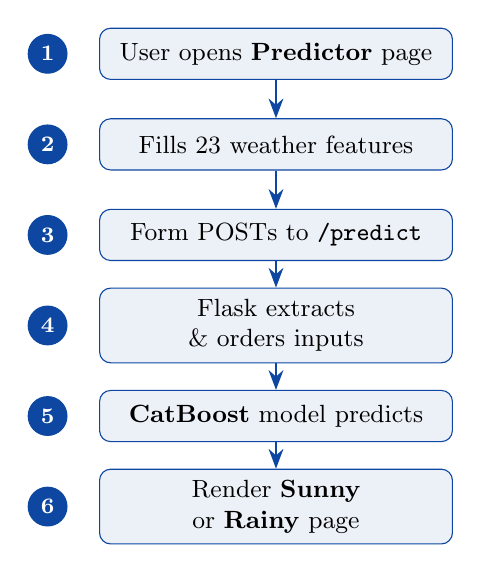
\begin{tikzpicture}[
        box/.style={rectangle, rounded corners=4pt, draw=deepblue, fill=deepblue!8,
                    text width=4.2cm, minimum height=0.65cm, align=center,
                    font=\small, inner sep=4pt},
        arrow/.style={-{Stealth[length=2.5mm]}, thick, deepblue},
        num/.style={circle, draw=deepblue, fill=deepblue, text=white,
                    font=\footnotesize\bfseries, inner sep=1.5pt, minimum size=14pt}
      ]
        \node[box] (A) at (0, 0)     {User opens \textbf{Predictor} page};
        \node[box] (B) at (0,-1.15)  {Fills 23 weather features};
        \node[box] (C) at (0,-2.3)   {Form POSTs to \texttt{/predict}};
        \node[box] (D) at (0,-3.45)  {Flask extracts \& orders inputs};
        \node[box] (E) at (0,-4.6)   {\textbf{CatBoost} model predicts};
        \node[box] (F) at (0,-5.75)  {Render \textbf{Sunny} or \textbf{Rainy} page};

        \node[num, left=0.4cm of A] {1};
        \node[num, left=0.4cm of B] {2};
        \node[num, left=0.4cm of C] {3};
        \node[num, left=0.4cm of D] {4};
        \node[num, left=0.4cm of E] {5};
        \node[num, left=0.4cm of F] {6};

        \draw[arrow] (A) -- (B);
        \draw[arrow] (B) -- (C);
        \draw[arrow] (C) -- (D);
        \draw[arrow] (D) -- (E);
        \draw[arrow] (E) -- (F);
      \end{tikzpicture}
    \end{column}
    % Right: tech stack
    \begin{column}{0.38\textwidth}
      \begin{block}{Frontend}
        HTML5, CSS3, Bootstrap~5, Jinja2
      \end{block}
      \vspace{0.3em}
      \begin{block}{Backend}
        Python, Flask, Flask-CORS
      \end{block}
      \vspace{0.3em}
      \begin{block}{ML Stack}
        CatBoost, scikit-learn, SMOTE, Pandas, NumPy
      \end{block}
      \vspace{0.3em}
      \begin{block}{Deployment}
        Gunicorn / local dev server
      \end{block}
    \end{column}
  \end{columns}
\end{frame}

% -------------------- Slide 7: Web Application --------------------
\begin{frame}{Web Application}
  \small
  \begin{columns}[T]
    \begin{column}{0.48\textwidth}
      \textbf{Landing Page}
      \begin{itemize}\setlength\itemsep{2pt}
        \item Home, About, Dashboard (9 charts + Power BI), Developer sections.
        \item Responsive navigation with hamburger menu on mobile.
      \end{itemize}
      \vspace{0.3em}
      \textbf{Predictor Page}
      \begin{itemize}\setlength\itemsep{2pt}
        \item Bootstrap~5 form with dropdowns for categorical fields.
        \item 49 location options, 16 wind directions, date picker.
      \end{itemize}
    \end{column}
    \begin{column}{0.48\textwidth}
      \textbf{Result Pages}
      \begin{itemize}\setlength\itemsep{2pt}
        \item \textcolor{orange}{\textbf{Sunny}} --- warm yellow gradient.
        \item \textcolor{blue}{\textbf{Rainy}} --- cool blue gradient.
      \end{itemize}
      \vspace{0.3em}
      \textbf{Prediction Flow}
      \begin{enumerate}\setlength\itemsep{2pt}
        \item User fills weather parameters.
        \item Form POSTs to \texttt{/predict}.
        \item Flask extracts \& orders 23 features.
        \item CatBoost returns 0 (sunny) or 1 (rainy).
        \item Corresponding result page rendered.
      \end{enumerate}
    \end{column}
  \end{columns}
\end{frame}

% -------------------- Slide 8: Conclusion & Future Work --------------------
\begin{frame}{Conclusion \& Future Work}
  \begin{columns}[T]
    \begin{column}{0.48\textwidth}
      \textbf{Summary}
      \begin{itemize}\setlength\itemsep{3pt}
        \item End-to-end \textbf{next-day rainfall prediction} for 49 Australian stations.
        \item Thorough preprocessing: imputation, outlier capping, encoding, SMOTE.
        \item Compared 7 models; \textbf{CatBoost} selected for deployment.
        \item Delivered as an interactive \textbf{Flask web app}.
      \end{itemize}
    \end{column}
    \begin{column}{0.48\textwidth}
      \textbf{Future Enhancements}
      \begin{itemize}\setlength\itemsep{3pt}
        \item Real-time weather API integration.
        \item Probability scores alongside predictions.
        \item Multi-day forecasting (2--7 days).
        \item Cloud deployment (AWS / Render).
        \item Deep learning models (LSTM / Transformer).
        \item Explainability via SHAP / LIME.
      \end{itemize}
    \end{column}
  \end{columns}
\end{frame}

% -------------------- Slide 9: Thank You --------------------
\begin{frame}{}
  \vfill
  \centering
  
\includegraphics[height=1.8cm]{images/bu_logo.png}\\[1em]
  {\Huge\textcolor{deepblue}{\textbf{Thank You!}}}\\[1em]
  {\Large Questions?}
  \vfill
\end{frame}

\end{document}
